\chapter{Design and Implementation}\label{chap:imp}

\section{Overview}

This chapter discusses the requirements of the software intended to analyse e-mails, the design of the program and its specifications, and finally the implementation itself.


    \section{Aims and Objectives}

    The software should
    automatically extract information from e-mail headers and analyse its results to
    display the personal information continaed within an e-mail's header, as well as
    information about the software configurations that may be found on a user's
    computer, or the servers used to send their e-mail.

    The program would be expected to satisfy the following minimal requirements
    in order for it to be considered successful: \begin{description} \item
    [{Accuracy}] --- any information produced by the parser should be reflective
    of the input e-mail

    \item [{Representation}] --- the produced visualisation should be intuitive
    to read: each element should be presented separately from the others, and
    clearly labelled.

    \item [{Portability}] --- the visual output produced by the program should
    be available to the user in a variety of formats.

    \item [{Interactivity}] --- the program should produce sensible warnings
    when an e-mail that is not possible to parse has been entered.
  \end{description}

  \section{Comparisons to Existing Software}

  \paragraph{Google and Microsoft Header Analysers} Both of the tools discussed in Sections~\ref{sec:goo} and~\ref{sec:mic} produced detailed information on the servers that are being used to send and received messages, with Google's tool also clearly reporting when its own servers were used to send a message.  The software should mimic this by providing a similar level of detail on the devices being used to send information, and extend this by looking up information on the device's owning organisation.  Additionally, a more exhaustive search of the other fields should be conducted, so more information about the sender can be provided than the immediately available details such as time, sender's e-mail and recipient.

  \paragraph{MITRE CVE Lookup and Norton Vulnerability Protection} The tools discussed in Sections~\ref{sec:mit} and~\ref{sec:nor} are both targeted at very different demographics.  The MITRE CVE Lookup is designed for IT progressionals and system administrators wishing to gather more information about specific vulnerabilities and software, requiring knowledge of the software present on a network or device.  The information presented is also not structured or sorted in a clear fashion.

  Norton's tool, on the other hand, is focused on individual users who administer their own systems.  The information is presented in such a way as to warn them as to which software needs updating or patching against a vulnerability, but provides few details on the nature of the vulnerabilities.

  The tool that is described in this report ought to be able to bridge the gap between these two tools, providing a useful and relevant list of vulnerabilities, without overloading the information provided, or requiring complex search terms to be crafted. 

  \section{Typical Use}

  On starting the application, the user will provide an e-mail that they wish
  to have analysed.  This will then be parsed, and some relevant information
  presented in a table.

  Lastly, an option is available to view the information about security
  vulnerabilities in a separate webpage, forming the main output of the
  program.

  The resultant webpage will be structured as in table~\ref{tab:format}.  It
  will then be possible for the user to click on the representations of the
  devices to find out more information.  It will also be possible to search
  within the vulnerability list to find more information, as well as filter by
  impact and availability details.

  \begin{table}[] \centering \begin{tabular}{@{}clllll@{}} \toprule
    \multicolumn{6}{c}{Email Header Information}                                                                                                                                                                                                                                      \\
    \midrule \multicolumn{2}{l}{\begin{tabular}[c]{@{}l@{}}Sender Information\\
    (Name, originating domain)\end{tabular}} & \multicolumn{2}{l}{Sender
    Software} & \multicolumn{2}{l}{\begin{tabular}[c]{@{}l@{}}Sender Usernames\\
    (Presented as a list with likely organisation)\end{tabular}} \\
    \multicolumn{6}{c}{Graphical representation of devices used to deliver the
    e-mail}                                                                                                                                                                                                \\
    \multicolumn{6}{c}{List of derived information including found software and
    similar information}                                                                                                                                                                                  \\
    \multicolumn{6}{c}{Histograms for vulnerability scores, separated by
    product}                                                  \\
    \multicolumn{6}{c}{Searchable and filterable table of discovered CVEs}                                                                                                                                                                                                            \\
    \bottomrule \end{tabular} \caption{Format of presented data found in e-mail
    header}\label{tab:format} \end{table}

\section{Program Overview}

The program is split up into three main stages: textual analysis and parsing; header contents analysis, and visualisation, as shown in Figure~\ref{fig:con}.  The relevant data is often stored in a central \texttt{MainWindow} class, rather than passed as a parameter, as the composition would indicate, allowing clear references to be maintained.

The  analysis is implemented as a series of stages, firstly, the e-mail header
is parsed, to extract important information to a predefined set of Java objects.
This is followed by the analysis phase, where the resultant data is passed to a
set of analyser modules, each running separately.  Finally, this information is
presented to the user.  After discussing an overview of each module, this chapter 
presents each of these stages in detail.

\begin{figure}
	\centering
\resizebox{0.9\textwidth}{!}{
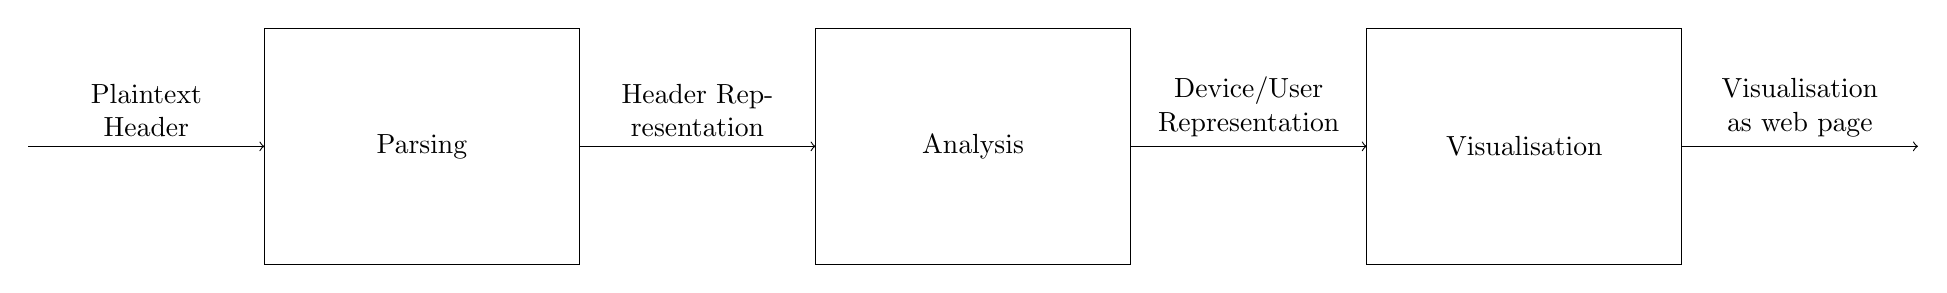
\begin{tikzpicture}
	\draw [->] (-3,1.5) -- (0,1.5) node [above, text width=2.5cm, align=center, midway] { Plaintext Header };
	\draw (0,0) rectangle node {Parsing} (4,3);
	\draw [->] (4,1.5) -- (7,1.5) node [above, text width=2.5cm, align=center, midway] { Header Representation };
	\draw (7,0) rectangle node {Analysis} (11,3);
	\draw [->] (11,1.5) -- (14,1.5) node [above, text width=2.5cm, align=center, midway] { Device/User Representation };
	\draw (14,0) rectangle node {Visualisation} (18,3);
	\draw [->] (18,1.5) -- (21,1.5) node [above, text width=2.5cm, align=center, midway] { Visualisation as web page };
\end{tikzpicture}}
\caption{Simplified Control Flow of Application}
\label{fig:con}
\end{figure}

\subsection{Parsing}

This module receives the plain-text of the e-mail as an input, splitting it into two sections, fields with the ``Received'' tag, and all other fields.  These are then parsed separately.  The other fields are easier to parse, as they can be loaded into a hashmap, split by the colon.  The trace fields require a more complex parsing strategy, fully described in Section~\ref{sec:par}.  This information is then extracted to more abstract Java objects, allowing the relevant information to be queried on a device-by-device basis, rather than constantly referring back to the source text.

\subsection{Analysis}

The analysis of the e-mail headers is handled independently by a number of small classes, each running asynchronously.  The decision was made to structure the program in such a way that concurrent operaton was possible in order to prevent blocking operations from limiting the progress of other operations. This also required care to ensure the separation between the model of the header and the model of the available information was maintained, as no guarantees could be placed on which thread was modifying data.

It is in this part of the program that the automated discovery of vulnerabilities takes place.  An example software configuration string is \texttt{cpe:/a:cloudbees:jenkins:2.2}, so it is necessary to attempt to convert found software information.  For example, \texttt{Apple Mail} would become \texttt{apple:mail} and a search would be performed over the database for configurations containing that string.


\subsection{Visualisation}

\section{Definitions}

The following covers the essential definitions required for the notation and
concepts that will be discussed in this document.

\subsection{Parsing}

In order to aid the parsing of the e-mail header, a combination of regular
expressions and context-free grammars are needed, and defined as follows.

\paragraph{Alphabets and Languages}

A set of symbols, usually denoted as $\Sigma$.  A language is a subset of
$\mathcal P (\Sigma)$.

The following special classes are provided as part of the Perl-Compatible
Regular Expression library, and are subsets of the alphabet of Unicode
characters, defined in~\cite{php_group_gutmans_lerdorf_suraski_boerger}.

\begin{description}

\item[alnum] --- letters and digits

\item[alpha] --- letters

\item[ascii] --- the set of ASCII characters (character codes 0 --- 127)

\item[blank] --- tabs or blank spaces

\item[cntrl] --- control characters

\item[digit] --- decimal digits

\item[graph] --- printing characters (excluding spaces)

\item[lower] --- lower-case letters

\item[print] --- printing characters (including spaces)

\item[punct] --- punctuation marks (printing characters excluding letters and spaces)

\item[space] --- white space

\item[upper] --- upper case letters

\item[word] --- ``word'' characters (same

\item[xdigit] --- hexadecimal digits

\end{description}
\subsubsection{Regular Languages}
Regular languages are defined as follows:
\begin{itemize}
\item $\emptyset$ and $\{\epsilon\}$ are regular languages
\item for each $a\in\Sigma$, $\{a\}$ is a regular language
\item if $A$ and $B$ are both regular, $A\cup B$, $A\cdot B$ and $A^*$ are regular languages.
\subitem{ $A\cup B$ is the union of two languages.  $A\cup B = \{s : s\in A \lor s \in B\}$}
\subitem{ $A\cdot B$ is the concatentation of two languages.  $A\cdot B = \{ ab : a \in A, b \in B\}$}
\subitem{ $A^*$ is the Kleene star of a language.}
\begin{align*}
    A_0&=\{\epsilon\}\\
    A_1&= A\\
    A_{i+1} &= \{ aa' : a \in A_i, a'\in A\}\\
    A^* &= \bigcup_{i\in\mathbb N} A_i
\end{align*}
\end{itemize}

\subsubsection{Context-Free Grammars}
A context-free grammar $G$ is defined as $G=\left(V,\Sigma, R,S\right)$ where:
\begin{itemize}
\item $V$ is a variable.
\item $\Sigma$ is the alphabet of symbols.
\item $R$ is a relation defined over $V\rightarrow \left(V\cup\Sigma\right)^*$
\item $S$ is the start symbol
\end{itemize}

For example, $\langle \text S \rangle$ is the field name with the associated
productions $\langle \text T \rangle \, \langle \text U \rangle$, where $T$ and
$U$ are productions.

\begin{bnf*}
	\bnfprod{S}{\bnfpn{T} \bnfsp{} \bnfpn{U}}
\end{bnf*}

For example, $\langle \text S \rangle$ is the field name with the associated
productions $a \, \langle \text U \rangle$, where $a$ is a terminal symbol.

\begin{bnf*}
	\bnfprod{S}{\bnftd{a} \bnfsp{} \bnfpn{U}}
\end{bnf*}
This is then extended in the following ways used in the RFC syntax.

The square brackets are used to indicate an optional element.
\begin{bnf*}
\bnfprod{field}{\bnfpn{field-name} \bnfts{:} \bnfsp{}[ \bnfpn{field-body} ]\bnfsp{} \bnfts{CRLF}}\\
\end{bnf*}

The asterisk is used to indicate an element that appears 0 or more times. $n*$
is used to indicate a component that repeats $n$ or more times.

\begin{bnf*}
\bnfprod{fields}{\bnfpn{dates}\bnfsp \bnfpn{source} \bnfsp 1\!*\bnfpn{destination} \bnfsp * \bnfpn{optional-fields}}\\
\end{bnf*}

The hash-symbol is used to indicate an element that appears a certain number of
times. $m*n$ is used to indicate a component that repeats at least $m$ times and
at most $n$ times.

\begin{bnf*}
\bnfprod{fields}{\bnfpn{dates}\bnfsp \bnfpn{source} \bnfsp 1\!\#\bnfpn{destination} \bnfsp * \bnfpn{optional-fields}}\\
\end{bnf*}

The $|$ is used to indicate a selection between a pair of elements.
\begin{bnf*}
\bnfprod{fields}{\bnfts{a}\bnfor \bnfts{b}}\\
\end{bnf*}

\subsection{Database Queries}
The following notations will be used for the CVE database queries.

\paragraph{Set-Theoretic Operators}
The operators $F\cup G$, $F \cap G$, $F\setminus G$ behave as is expected for
these operators, resulting in the union, intersection and difference of the
sets.  The only proviso being that the atrribute names must match.

\paragraph{Selection} \[\sigma_{\text{product}=\text{thunderbird}}D\]
The above notation is used to indicate a search over the attribute named
``product'' for the string ``thunderbird'' in the database table $D$.  As a
single database is only being used, this may be occasionally elided.  The output
of this function is another object of the same type as $D$.

\paragraph{Projection}
\[\pi_{\text{product}}D\]
The above notation is used to indicate a projection on the attribute named
``product'' in the database table $D$.  The output of this function is another
object of the same type as $D$.

\paragraph{Composition}
The above functions results can be coposed repeatedly to produce more specific
search queries.

\subsection{Data Structures}
These wil be drawn using square boxes to represent single objets that are encapsulated
within an object.  Square boxes with an inner square box indicate some collection
of objects.

Thin arrows will be used to denote the encapsulation relation, with thicker
arrows being used to list relevant public methods.

Where the type of an object can be expressed simply, the following conventions are used:
\begin{description}
	\item [Functions] --- $\alpha \rightarrow \beta \, \texttt{Str}$ is a function from $\alpha$ to $\beta$ stored using a \texttt{Str} object in Java.
	\item [Tuples] --- $(\alpha, \beta)$ represents a two-tuple containing objects of type $\alpha$ and $\beta$, respectively.  This extends naturally for arbitrarily many objects.
	\item [Lists] --- $[\alpha]$ represents a list or array of objects, all with type $\alpha$.
\end{description}

\section{Data Extraction and Parsing}

The parser's operation completes in a number of stages, following RFC822
(\cite{RFC0822}).  The header is divided up into two disjoint sections, the
routing information (\texttt{Received from...}) and the key-value map of other
pertinent information.

\subsection{Received fields}\label{sec:par}

The received fields are the most complicated part of the e-mail header to parse,
as they are described by a non-trivial grammar, presented below.

\begin{bnf*}
\bnfprod{message}{\bnfpn{fields}\bnfsp *(\bnfts{CRLF} \bnfsp *\bnftd{text})}\\
\bnfprod{fields}{\bnfpn{dates}\bnfsp \bnfpn{source} \bnfsp 1\!*\bnfpn{destination} \bnfsp * \bnfpn{optional-fields}}\\
\bnfprod{field}{\bnfpn{field-name} \bnfts{:} \bnfsp [ \bnfpn{field-body} ]\bnfsp \bnfts{CRLF}}\\
\bnfprod{field-name}{\bnftd{any word consisting of CHAR, excluding CTLs, SPACE, and ``'':''}} \\
\bnfprod{field-body}{\bnfpn{field-body-contents} \bnfsp [\bnfts{CRLF} \bnfsp \bnftd{LWSP-char}\bnfsp  \bnfpn{field-body}]}\\
\bnfprod{field-body-contents}{\bnftd{ASCII characters}}\\
\bnfprod{source}{[\bnfpn{trace}] \bnfsp \bnfpn{originator} [\bnfpn{resent}]}\\
\bnfprod{trace}{\bnfpn{return}\bnfsp 1\!* \bnfpn{received}}\\
\bnfprod{return}{\bnfts{Return-path:}\bnfsp{} \bnfpn{route-addr}}\\
\bnfprod{recieved}{\bnfts{Received:}}\\
\bnfprod{cont.}{[\bnfts{from}\bnfsp\bnfpn{domain}]}\\
\bnfprod{cont.}{[\bnfts{by}\bnfsp\bnfpn{domain}]}\\
\bnfprod{cont.}{[\bnfts{via}\bnfsp\bnfpn{atom}]}\\
\bnfprod{cont.}{*(\bnfts{with}\bnfsp\bnfpn{atom})}\\
\bnfprod{cont.}{[\bnfts{id}\bnfsp\bnfpn{msg-id}]}\\
\bnfprod{cont.}{[\bnfts{for}\bnfsp\bnfpn{addr-spec}]}\\
\bnfprod{cont.}{\bnfts{;}\bnfsp\bnfpn{date-time}}\\
\bnfprod{msg-id}{\bnfts{$<$}\bnfpn{addr-spec}\bnfts{$>$}}\\
\bnfprod{addr-spec}{\bnfpn{local-part}\bnfsp\bnfts{@}\bnfsp\bnfpn{domain}}\\
\bnfprod{local-part}{\bnfpn{word}\bnfsp *(\bnfts{.}\bnfsp\bnfpn{word})}\\
\bnfprod{word}{\bnfpn{atom}\bnfor\bnfpn{quoted-string}}\\
\bnfprod{domain}{\bnfpn{sub-domain} *(\bnfts{.}\bnfpn{sub-domain})}\\
\bnfprod{sub-domain}{\bnfpn{domain-ref}\bnfor\bnfpn{domain-literal}}\\
\bnfprod{domain-ref}{\bnfpn{atom}}\\
\bnfprod{date-time}{[ \bnftd{day,} ] \bnfsp \bnftd{date}\bnfsp \bnftd{time}}\\
\bnfprod{atom}{1\!*\bnftd{any character excluding specials, SPACE and CTLs}}\\
\end{bnf*}

An example field is as follows:
\begin{verbatim}
Received: from relay12.mail.ox.ac.uk (129.67.1.163)
    by HUB05.ad.oak.ox.ac.uk (163.1.154.231)
    with Microsoft SMTP Server id 14.3.169.1;
    Sat, 14 Nov 2015 10:55:35 +0000
\end{verbatim}

Of particular interest is the pair of hostnames (both are needed as each line is analysed independently, therefore it is not necessary to treat the last line as a special case) and their associated IP addresses.  The hostname is of more interest, as performing an IP address lookup is less complicated than determining a hostname.  The software used is identified by the \texttt{with} field, and is also of interest, however, is insufficient in most cases to produce meaningful CVE data.

\subsection{Other fields}

These are read by a Python script and output to \texttt{STDOUT} to be read by
the Java parser in a consistent format.  These are then loaded into a hashmap to
allow quick lookup.


\subsection{Input Data Structures}
The raw string of the message header is the only input to this module.

\subsection{Output Data Structures}
The data structure presented in Figure~\ref{fig:hea} shows the output of the
parsing and textual analysis module, which is then provided as an input to the
analysis modules.

\begin{figure}
\centering
\resizebox{0.9\textwidth}{!}{
	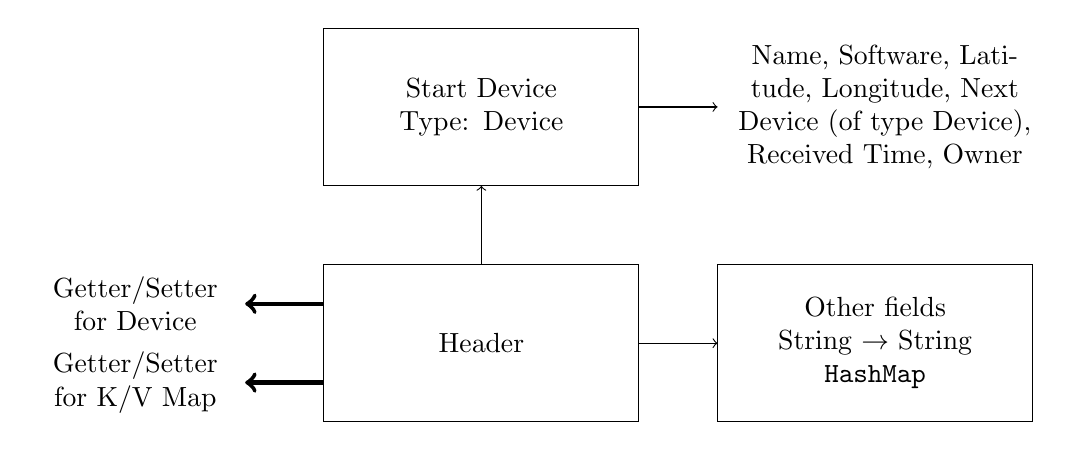
\begin{tikzpicture}
		\draw (0,0) rectangle node {Header} (4,2);
		\draw (0,3) rectangle node [text width = 3.5cm, align=center] {Start Device\\Type: Device} (4,5);
		\draw (5,0) rectangle node [text width = 3.5cm, align=center]
		{Other fields\\String $\rightarrow$ String \\ \texttt{HashMap}} (9,2);
		\draw [->] (2,2) -- (2,3);
		\draw [->] (4,1) -- (5,1);
		\draw [->] (4,4) -- (5,4) node [right, text width = 4cm,align=center] { Name, Software, Latitude, Longitude, Next Device (of type Device), Received Time, Owner};
		\draw [->, ultra thick] (0,1.5) -- (-1,1.5) node [left, text width = 2.5cm,align=center] { Getter/Setter for Device};
		\draw [->, ultra thick] (0,0.5) -- (-1,0.5) node [left, text width = 2.5cm, align=center] { Getter/Setter for K/V Map};
\end{tikzpicture}
	}
	\caption{Header Data Structure Format}
	\label{fig:hea}
\end{figure}


\section{Analysis}

After completing the parsing of the fields, it is then ready to be analysed for
different features.  All of the analysers implement the \texttt{HeaderAnalyser}
interface, requiring information about the header to be analysed, and the
currently running application.  All of these then implement the
\texttt{Runnable} interface, allowing the class to be run asynchronously.

\subsection{Text-Based}

The fields from the header are analysed in different modules, with searches
being performed for specific strings.  Of particular interest to Oxford Nexus
users is the ``X-Oxford-Username'' string, containing the username of the
individual that sent the message.  As confirming the username is a fairly
standard security procedure for an IT support technician, having access to this
information could allow a phisher in a later stage of an attack to increase
their credibility.

In some cases, the likely keys that are being searched for are known in advance,
and can then be checked against the hash-map of entries.

An example of this approach is for the specific check for an Oxford username, as shown in Algorithm~\ref{alg:oxf}.

\begin{algorithm}
	\KwIn{Header}
	\KwOut{Any username that is found}
$kws \gets \{\texttt{X-Oxford-Username}, \texttt{X-Username}, \texttt{X-Authenticated-User}\}$\;
\ForEach{$kw\in kws$}{
	\If{$kw\in$ Header.KvMap}{ \Return{Header.KvMap(kw)}\; }
}
	\caption{Lookup based on a known key}
	\label{alg:oxf}
\end{algorithm}

Alternatively, we may be interested in properties of the keys, necessitating a search over the keys, as shown in Algorithm~\ref{alg:exc}.

\begin{algorithm}
	\KwIn{Header}
	\KwOut{Any information relating to Microsoft Exchange that is found}
	\ForEach{Key $k\in $ Header.KvMap}{
		\If{$k$ starts-with \texttt{X-MS-Exchange}}{
			\Return{Header.KvMap($k$)}\;
		}
	}
	\caption{Lookup based on a key property}
	\label{alg:exc}
\end{algorithm}

\subsection{Client Inferrence}

In \cite{nurse2015investigating}, a number of different e-mail clients were identified based on the header tags that were present. By identifiying these pieces of software likely to be found on a user's machine, we gain a significant amount of information from them, and should therefore devote some effort to correctly identifying them.  Using a number of e-mail samples provided, I have been able to extract examples for a number of different e-mail clients, and use them to infer the client being used.  Using a sample of e-mails, it is possible to find information for additional e-mail clients and senders, such as (but not limited to) PHPMailer and Foxmail.  A number of these approaches are shown in Algorithm~\ref{alg:inf}.

\begin{algorithm}
	\KwIn{Header}
	\KwOut{The name of the software that is likely being used, and necessary CVE Product name (elided for brevity)}
	\uIf{``Message-ID''${}\in{}$Header.KvMap}{
		\If{Header.KvMap(``Message-ID'') contains ``email.android.com''}{
			\Return{``Android Device''}\;
		}
	}
	\uElseIf{``X-Mailer''${}\in{}$Header.KvMap}{
		\Switch{Header.KvMap(``X-Mailer'') contains}{
			\Case{``iPhone''}{\Return{``iPhone''}}
			\Case{``Outlook Express''}{\Return{``Microsoft Outlook Express''}}
			\ldots
		}
	}
	\uElseIf{``User-Agent''${}\in{}$Header.KvMap}{
		\Return{``Thunderbird''}\;

	}
	\ElseIf{Header.KvMap${}\cap{}$OutlookKeywords${}\neq\emptyset$}{
		\eIf{``X-Mailer''${}\in{}$Header.KvMap}{ \Return{Apple Mail}}{ \Return{Outlook}}

	}
	\caption{Client Inferrence Technique}
	\label{alg:inf}
\end{algorithm}


\subsection{Database Queries}

Using the results gathered from the text-based queries and analysis of the
received fields, relevant software configurations are extracted and queried
against results in the CVE database.  These are then parsed and collated in
preparation for displaying the outputs. Specifically, the queries are limited
to those matching the product name, and vulnerabilities that can be remotely
executed.

As more information is found, more details of products used will also become
available.  These are added asynchronously.

\begin{algorithm}
	\KwIn{Header product name $p$}
	\KwOut{CVE Entries}
	cve-list $\gets\emptyset$\;
	\ForEach{$s\in\sigma_{\text{vector}\neq\text{LOCAL}}\sigma_{\text{product}=p} D$}{
		cve-builder$\gets$blank cve\;
		cve-builder.id$\gets\pi_{\text{CVE-ID}} s$\;
		$\ldots$ -- extract other features\;
		cve-list $\gets$ cve-list${}\cup{}$make(cve-builder)\;
	}
	\Return{cve-list}\;
	\caption{Extracting CVE entries}
\end{algorithm}

\subsection{Analysis Modules and Data Flow}

The following modules are used in the analysis of e-mail headers. Via \texttt{HeaderAnalyser}, they all subclass \texttt{Callable<Object>}, allowing them to return values to calling classes when side-effects are undesirable.

\begin{description}
	\item[HeaderAnalyser] --- the base interface for all analysis modules.
	\item[ClientInferrer] --- as described in Algorithm~\ref{alg:inf}, this analyses the entire header, looking for specific indicators relating to e-mail clients.
	\item[DeviceAnalyser] --- Extracts the hostname, and then IP address, or IP address for each device, allowing a lookup of its co-ordinates.
	\item[ExchangeHeaderAnalyser] --- determines if a Microsoft Exchange server has handled the message.
	\item[GeoIPAnalyser] --- Given an IP address, this module looks up the latitude and longitude for said IP address.  This search will fail for local IP addresses (commonly found in the 192.168.0.0/16 subnet).
	\item[UsernameHeaderAnalyser] --- This module searches for the specific \texttt{X-Oxford-Username} field, one of the most common fields in my collection of e-mail headers, as well as a number of more generic username fields.
	\item[SenderInformationExtractor] --- This is used to lookup an individual's name from the set of fields, if it is available.
	\item[VulnerabilityAnalyser] --- For each entry from the database as a \texttt{String}, this analyser returns a \texttt{VulnerabilityDisclosure} object.
	\item[VulnerabilityFinderManager] --- this is an interface for other classes to implement. A reference implementation is provided in \texttt{VulnerabilityFinderManagerImpl}, with a simple implementation found in \texttt{NoopVulnerabilityFinderManager} for systems that lack the CVE database.
	\item[WhoIsAnalyser] --- Using a hostname, this looks up the relevant owning organisation for a server, if it is available.
\end{description}

Figure~\ref{fig:flo} shows the direct interaction of the analysis modules.  Unless noted, if an arrow goes from $\alpha$ to $\beta$, it is used to indicate that $\alpha$ calls $\beta$, passing data from $\alpha$, and/or receiving data from $\beta$.

\begin{figure}
	\resizebox{0.9\textwidth}{!}{
\begin{tikzpicture}
\tikzset{every node/.style={align=center, text width = 3.5cm, font = \ttfamily}}

\draw (0,0) rectangle node {Main Window} (4,2);
\draw [->] (4,1) -- (5,1);
\draw (5,0) rectangle node {Oxford Analyser} (9,2);
\draw [->] (4,2) -- (5,3);
\draw (5,3) rectangle node {Client Inferrer} (9,5);
\draw (0,-1) rectangle node {Exchange Header Analyser} (4,-3);
\draw [->] (2,0) -- (2,-1);
\draw (0,3) rectangle node {Device Analyser} (4,5);
\draw [->] (2,2) -- (2,3);
\draw (5,6) rectangle node {Vulnerabiltiy Finder Manager} (9,8);
\draw [->] (4,5) -- (5,6);
\draw [->] (7,5) -- (7,6);
\draw (10,6) rectangle node {Vulnerability Analyser} (14,8);
\draw [->] (9,7)  -- (10,7);
\draw (0, 6) rectangle node {GeoIP Analyser} (4,8);
\draw [->] (2,5) -- (2,6);
\draw (-5,0) rectangle  node {Sender Information Analyser} (-1,2);
\draw [->] (0,1)  -- (-1,1);
\draw (-1,6) rectangle node {WhoIs Analyser} (-5,8);
\draw [->] (0,5) -- (-1,6);
\end{tikzpicture}	
	}
\caption{Information flow between analysis modules}
\label{fig:flo}
\end{figure}

\subsection{Output Data Structures}

The output of the analysis modules is compiled into the \texttt{FoundInformation} class, which represents the list of facts, servers and other information that has been gathered from an e-mail.

\begin{figure}
	\centering
\resizebox{0.9\textwidth}{!}{%
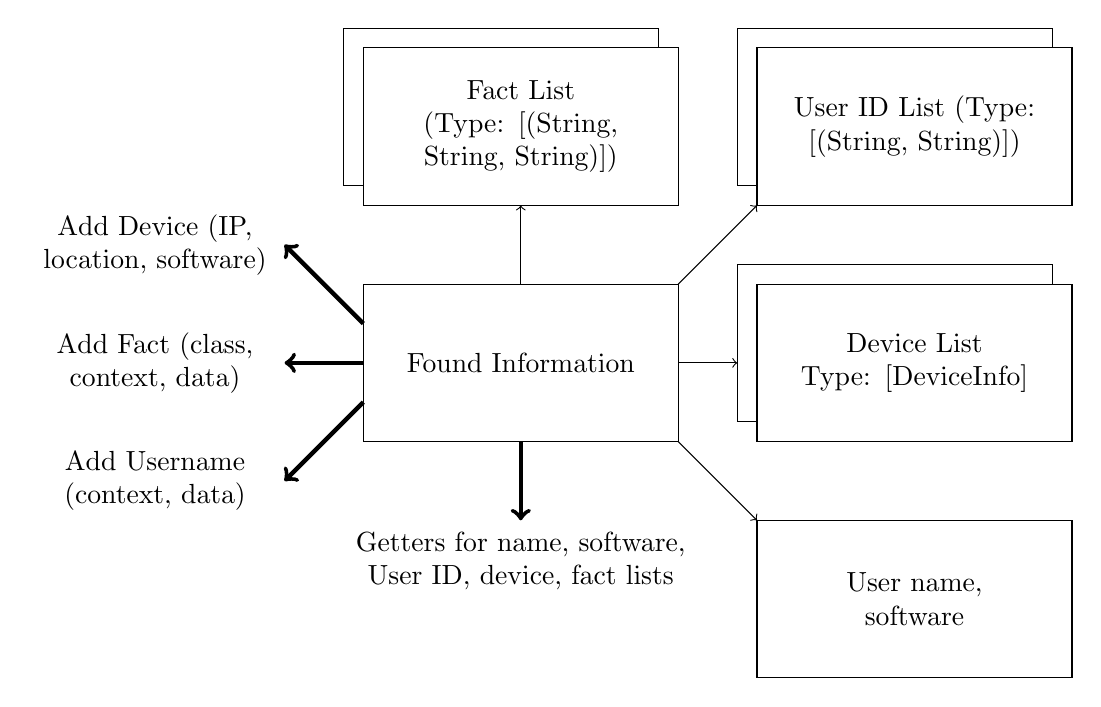
\begin{tikzpicture}
\draw (0,0) rectangle node {Found Information} (4,2);
\draw [->, ultra thick] (0,0.5) -- (-1,-0.5) node [left, text width = 3cm, align=center] {Add Username (context, data) };
\draw [->, ultra thick] (0,1) -- (-1,1) node [left, text width = 3cm, align=center] {Add Fact (class, context, data) };
\draw [->, ultra thick] (0,1.5) -- (-1,2.5) node [left, text width = 3cm, align=center] {Add Device (IP, location, software) };
\draw [->] (2,2) -- (2,3);
\draw [fill=white] (-0.25, 3.25) rectangle  (-0.25+4, 3.25+2);
\draw [fill=white] (-0, 3) rectangle node [text width = 3.5cm, align=center] {Fact List\\(Type: [(String, String, String)])} (-0+4, 3+2) ;
\draw [fill=white] (-.25+5, 3.25) rectangle (-0.25+5+4, 3.25+2);
\draw [fill=white] (5, 3) rectangle node [text width = 3.5cm, align=center] {User ID List (Type: \\{} [(String, String)])} (5+4, 3+2);
\draw [->] (4,2) -> (5,3);
\draw [fill=white] (-0.25+5, 0.25) rectangle (8.75, 2.25);
\draw [fill=white] (5, 0) rectangle node [text width = 3.5cm, align = center] {Device List\\ Type: [DeviceInfo]} (9, 2);
\draw [->] (4,1) -> (4.75,1);
\draw [->, ultra thick] (2,0) -- (2,-1) node [below, text width = 4.75cm, align = center] {Getters for name, software, User ID, device, fact lists};
\draw [->] (4,0) -> (5,-1);
\draw (5,-1) rectangle node [align=center] {User name,\\ software} (9,-3);
\end{tikzpicture}}
\caption{Found Information Data Structure Format}
\label{fig:fou}
\end{figure}

\begin{figure}
\centering
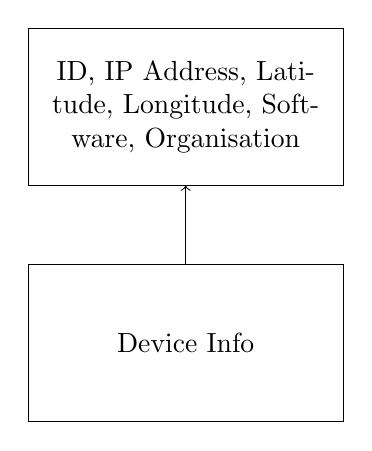
\begin{tikzpicture}
\draw (0,0) rectangle node {Device Info} (4,2);
\draw (0,3) rectangle node [align=center, text width = 3.5cm]{ID, IP Address, Latitude, Longitude, Software, Organisation} (4,5);
\draw [->] (2,2) -- (2,3);
\end{tikzpicture}
\caption{Device Information Data Structure}
\end{figure}

\section{Visualising the Results}

Using a pre-existing template, the results from the e-mail analysis will be
presented in a temporary webpage, which can then be saved independently.  Other
than the referenced JavaScript libraries, and a freely available set of country 
borders, the document requires no additional information or database access, 
allowing it to be quickly shared.

In order to export the results, the process described in Algorithm~\ref{alg:vis} are taken.  The \textit{keyword} objects refered to are one of a number of specific strings representing one of the sender's name, organisation, client or usernames; CVE entries, fact entries, products that have been found, or servers that have been found.

\begin{algorithm}
	\KwIn{Found Information Object}
	\KwOut{Webpage}
	$\textit{lines}\gets\text{read-lines(webpage-template)}$\;
	\ForEach{$l\in\text{lines}$}{
		\eIf{$l$ contains keyword}{
		$\textit{webpage}\gets_+ l[\text{field from FoundInformation}/\text{keyword}]$\;
		}{
		$\textit{webpage}\gets_+ l$\;
		}
	}
	\Return{webpage}\;
	\caption{Exporting the Found Information to Visualisations}
	\label{alg:vis}
\end{algorithm}
